\documentclass[t]{beamer}


% Appearance:

\usetheme{KTHprofile}
\usefonttheme[onlylarge]{structurebold}



% Standard packages
\usepackage{picture}
\usepackage[english]{babel}
\usepackage[latin1]{inputenc}
\usepackage{times}
\usepackage[T1]{fontenc}
\usepackage{lipsum}
\usepackage[]{epstopdf}
\usepackage[absolute,overlay]{textpos}
\usepackage{pifont}
\usepackage{subfig}
\graphicspath{{Results/}{Algorithm/}}

\title[Inisintiur sequi aliquia tis dis in para] 
{%
  Safe Learning for Control%
}

%\author{}

\author[Oskar, Friends]
{
Caroline Heidenreich
}

%\author[Dude, Friends]
%{
%The~Dude\inst{1} \and
%And~Friends\inst{2}
%}

\institute{}

%\institute[KTH Royal Institute of Technology]
%{\inst{1} KTH Royal Institute of Technology, Sweden\and
%\vskip-4mm
%\inst{2} KTH Royal Institute of Technology, Sweden
%}

\date{\today}


\begin{document}


\begin{frame}
\titlepage
\end{frame}

\iffalse
\begin{frame}
\frametitle{Contents}
\begin{itemize}
\item Motivation
\item Algorithm
\item Results
\item Conclusions and Future Work
\end{itemize}
\end{frame}
\fi

\begin{frame}
\frametitle{Motivation}
\framesubtitle{Why do we want to do safe learning in control?}
\begin{itemize}
\item Model-based control suffers often from poor model accuracy\\
$\Rightarrow$ Learning Control
\item But: Reinforcement learning algorithms not designed for satisfying constraints so we need an additional safety-preserving controller\\ $\Rightarrow$ Safe Learning Control
\end{itemize}

\end{frame}


\begin{frame}
\frametitle{Example}
\begin{itemize}
\item Autonomous vehicle with \linebreak partly known model
\item Task: learn control with reinforcement learning without driving off the road
\item To simplify, we only look at the truck's position
\end{itemize}
\begin{textblock*}{5cm}(8cm,4.79cm) % {block width} (coords)
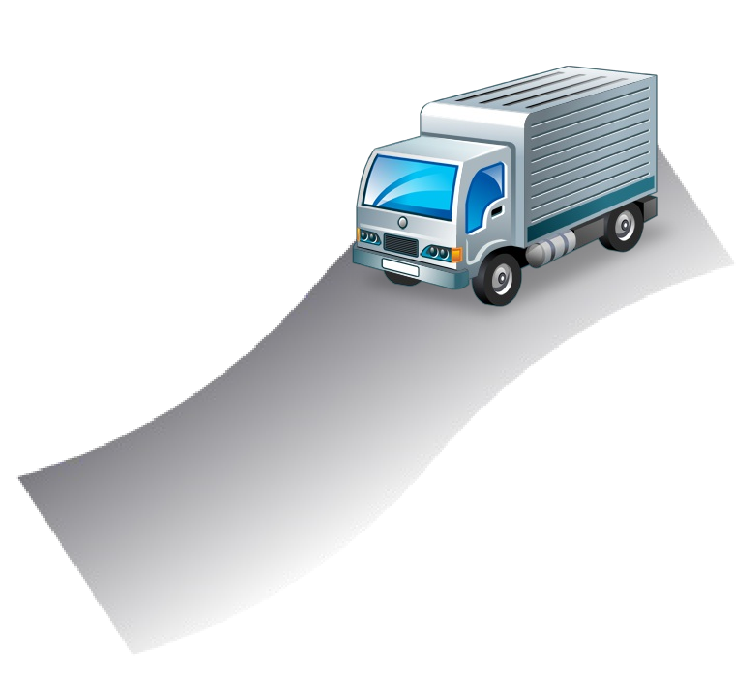
\includegraphics[width=0.29\paperwidth]{TruckOnStreet}
\end{textblock*}
\end{frame}



\begin{frame}
\frametitle{Algorithm}
\framesubtitle{Markov Decision Process}
\begin{itemize}
\item Discretise states and actions.
\item Assign rewards to each state-action pair.
\item Decide for an objective function that the agent should maximise.
\end{itemize}
\begin{textblock*}{7cm}(2.3cm,5.05cm) % {block width} (coords)
\small{Reward function}\\
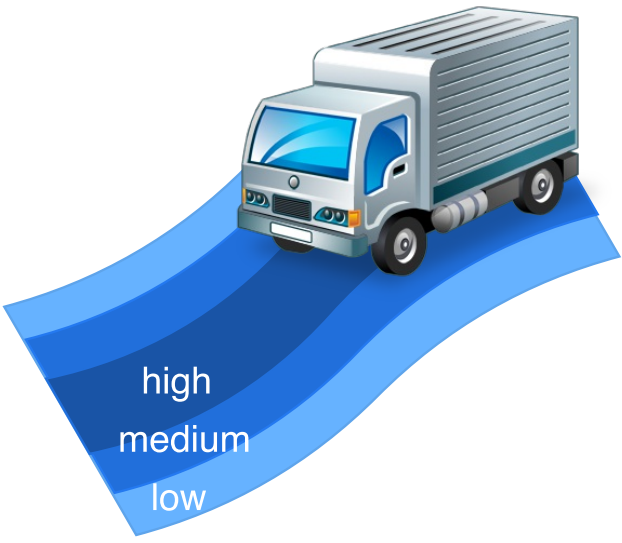
\includegraphics[trim=0mm 0mm 0mm 0mm, width=0.5\textwidth]{Reward}
\end{textblock*}
\begin{textblock*}{5cm}(7cm,5.05cm) % {block width} (coords)
\small{Objective function}
\end{textblock*}
\begin{textblock*}{5cm}(6.2cm,6.2cm) 
\begin{equation*}
\noindent
R_t = \sum_{k=0}^T\gamma^kr_{t+k+1}
\end{equation*}
\end{textblock*}
\end{frame}


\begin{frame}
\frametitle{Algorithm}
\framesubtitle{Reinforcement Learning}
General Idea: Finding the optimal policy by playing actions and receiving rewards
\begin{enumerate}
\item The agent chooses an action.
\item The agent receives an external reward.
\item The agent updates its policy dependent on the received reward.
\end{enumerate}
\vspace{0.5cm}
\ding{51} The policy will converge to the optimal policy.\\
\ding{55} No safety guarantees.
\begin{textblock*}{7cm}(9cm,5cm) % {block width} (coords)
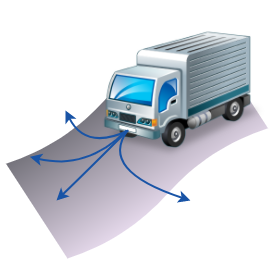
\includegraphics[trim=0mm 0mm 0mm 0mm, width=0.5\textwidth]{PossibleTrajectories}
\end{textblock*}
\end{frame}

\begin{frame}
\frametitle{Algorithm}
\framesubtitle{Safe Set Calculation}
How can we ensure safety with uncertain dynamics?
\begin{itemize}
\item We treat the unmodelled dynamics as a bounded disturbance.
\iffalse
\item We assume a worst-case disturbance driving the vehicle off the road and an optimal control trying to keep the vehicle in the middle of the road.
\item \textbf{safe} (no disturbance can manage to drive the vehicle off the road).
\item \textbf{unsafe} (there is a disturbance that manages to push the system off the road).

\fi
\item With Hamilton-Jacobi-Isaacs (HJI) reachability analysis, we can determine for each state if it is safe or not.
\end{itemize}

\begin{figure}
\vspace{-0.6cm}
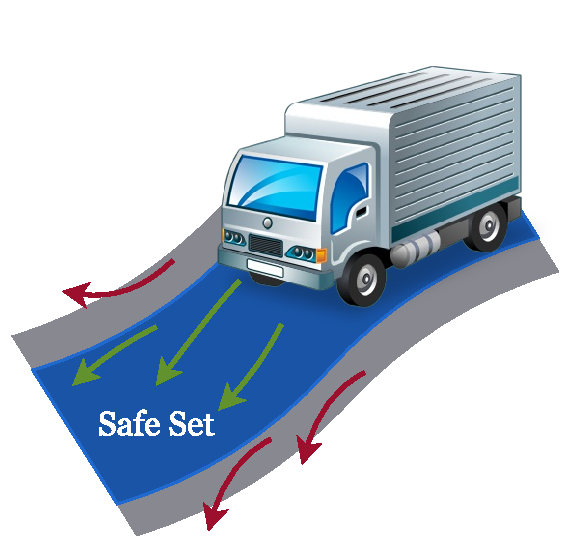
\includegraphics[clip, trim=3mm 3mm 4mm 10mm, width=0.38\textwidth]{SafeStreet}
\end{figure}

\end{frame}

\begin{frame}
\frametitle{Algorithm}
\framesubtitle{Safe Set Calculation}
\begin{itemize}
\item At the borders of the safe set: Apply safe control.
\item Within the safe set: Reinforcement learning.
\end{itemize}
\vspace{1cm}
\ding{51} Now we can learn a control without ever leaving the road.\\
\ding{55} The safe set might be very small due to a conservative initial disturbance estimate.
\end{frame}

\begin{frame}
\frametitle{Algorithm}
\framesubtitle{Disturbance Estimation with Gaussian Processes}
\begin{itemize}
\item Update the conservative initial disturbance range with Gaussian Process (GP) regression in the light of data.
\item GP regression: Non-parametric regression method that gives:
\begin{enumerate}[a.]
\item an estimate for the disturbance.
\item a measure how certain this estimate is.
\end{enumerate}
\end{itemize}
\end{frame}

\begin{frame}
\frametitle{Algorithm}
\framesubtitle{Summary of Approach}
\begin{textblock*}{9.9cm}(2cm,2.7cm) % {block width} (coords)
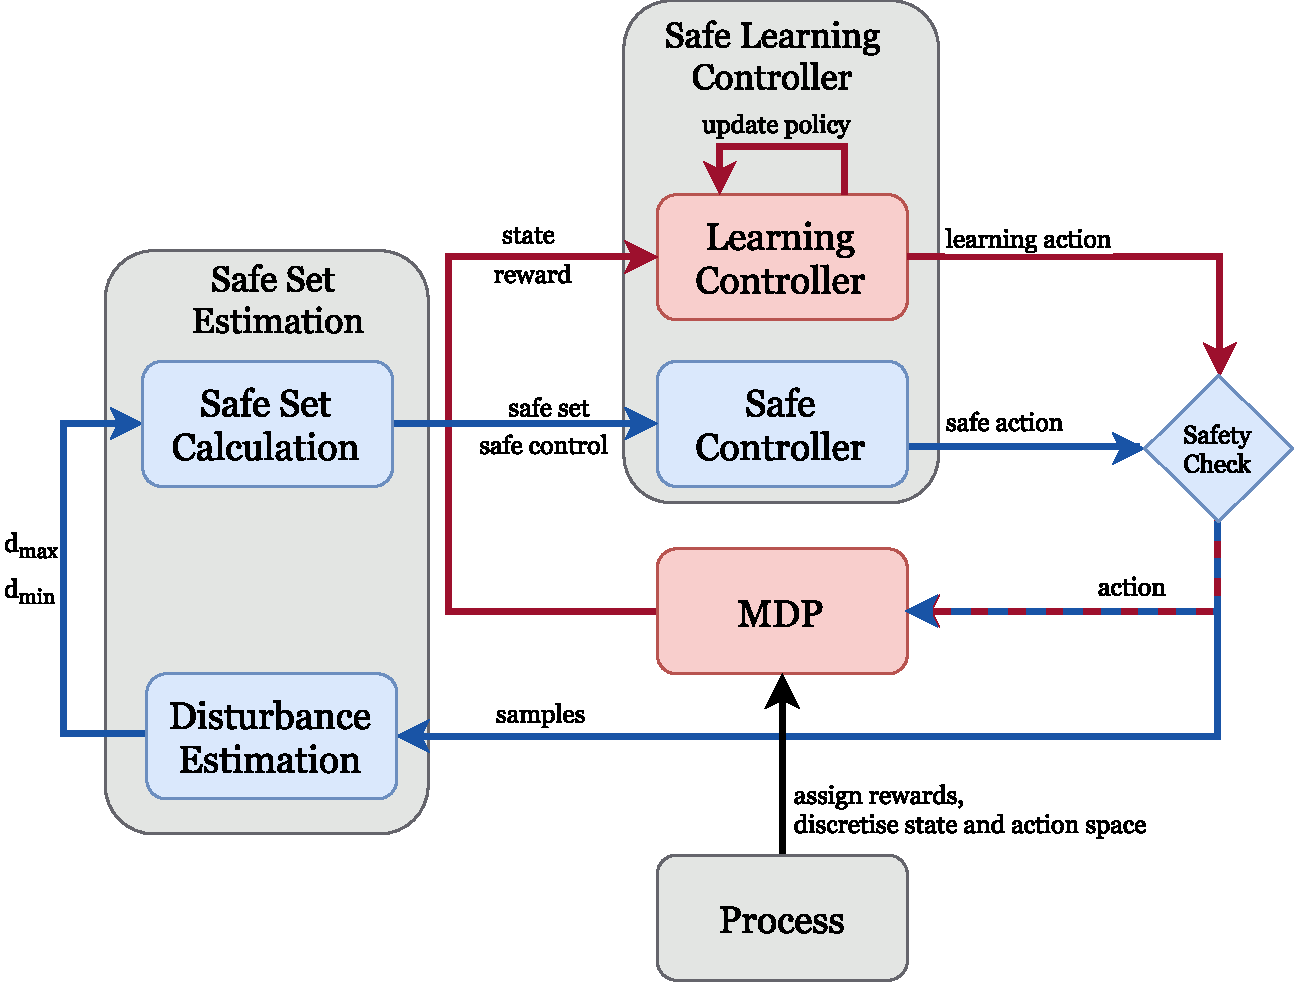
\includegraphics[trim=3mm 3mm 3mm 14mm, width=0.8\textwidth]{flow}
\end{textblock*}
\end{frame}

\begin{frame}
\frametitle{Algorithm}
\framesubtitle{Exploration}
\begin{itemize}
\item Trade-off between \linebreak exploration and \linebreak exploitation.
\item Our algorithm \\ incorporates \\ exploration explicitly \\ by employing \\ \textbf{Incremental} \\ \textbf{Q-learning}
\end{itemize}

\begin{textblock*}{8cm}(6cm,0.5cm) % {block width} (coords)
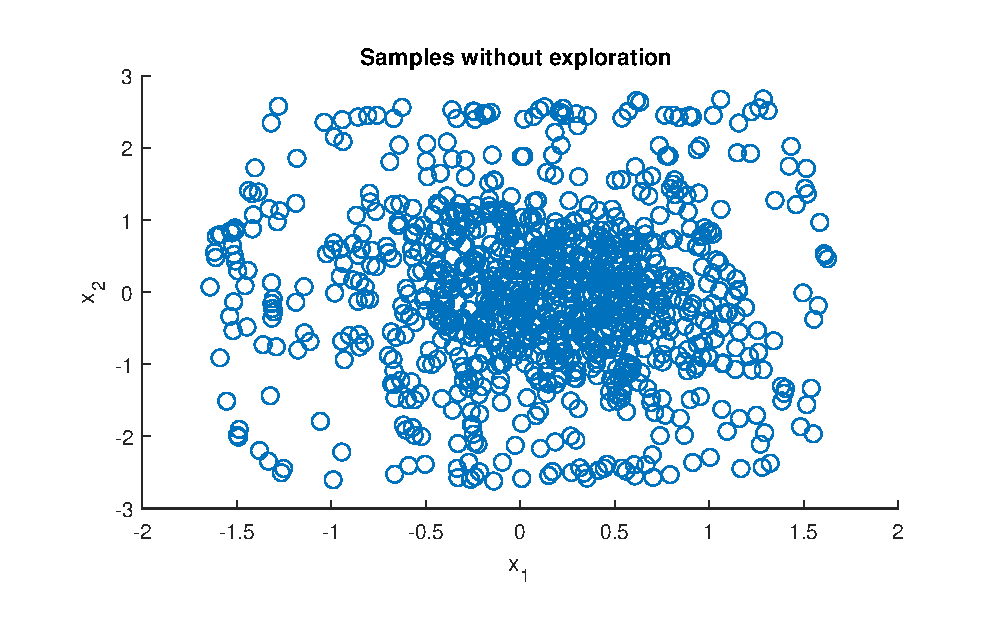
\includegraphics[width=0.8\textwidth]{Unexploration_samples}
\end{textblock*}
\begin{textblock*}{8cm}(6cm,4.3cm) % {block width} (coords)
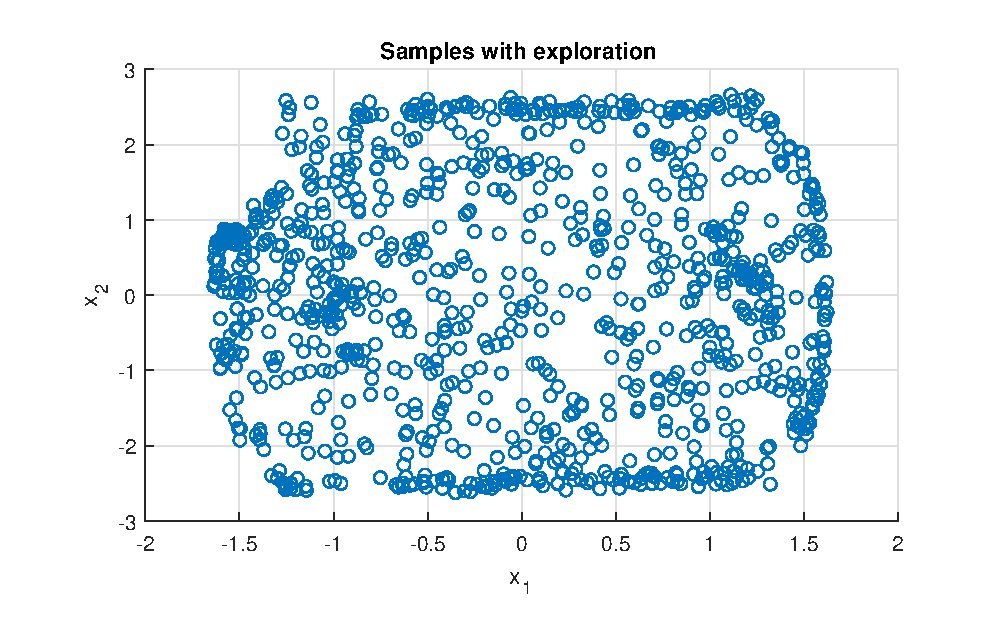
\includegraphics[width=0.8\textwidth]{Exploration_samples}
\end{textblock*}
%\begin{figure}
%\subfloat{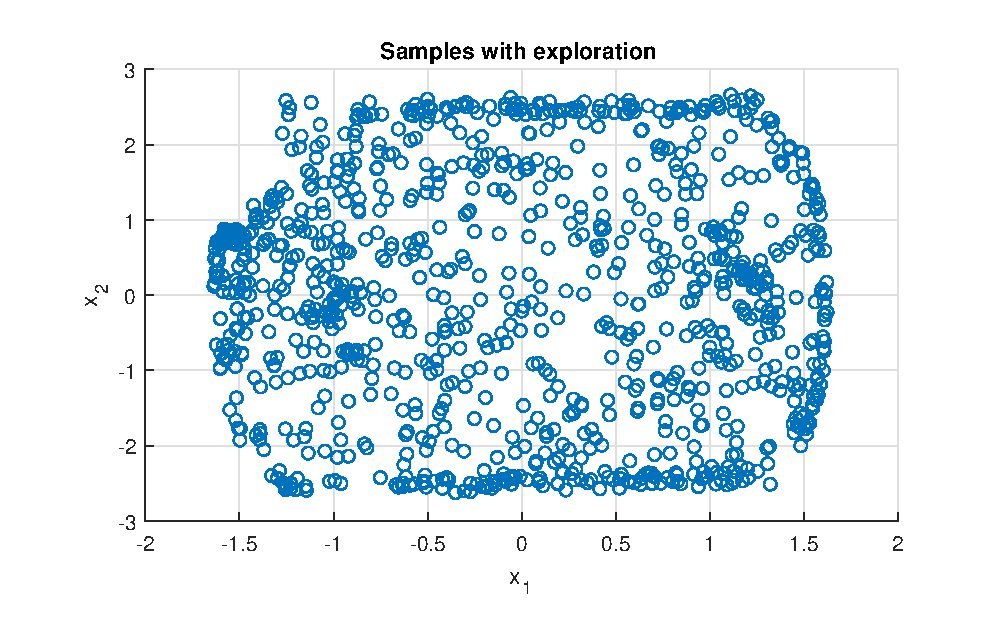
\includegraphics[width=0.5\textwidth]{Exploration_samples}}\qquad
%  \subfloat{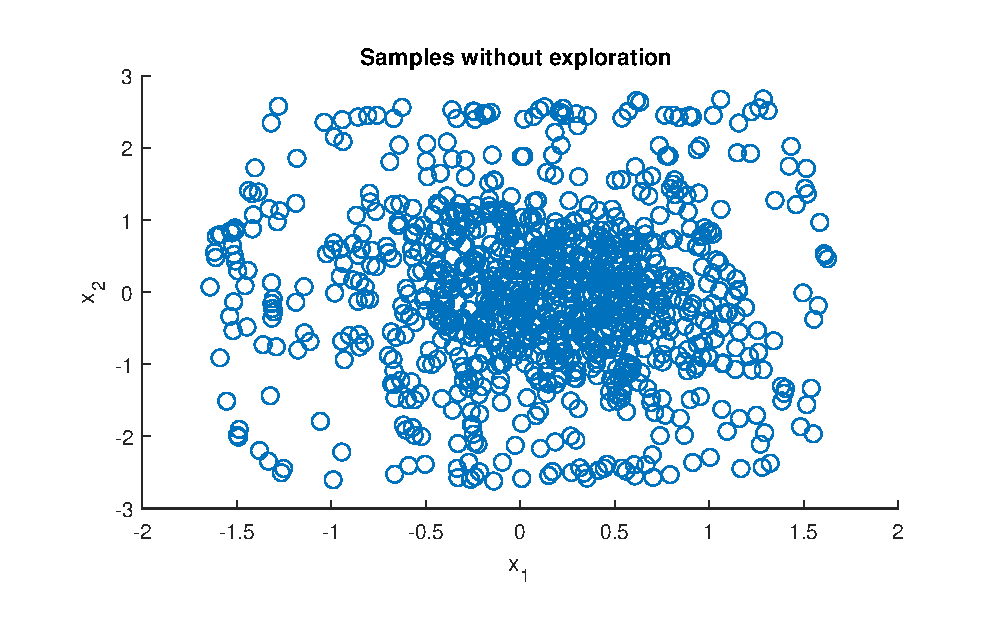
\includegraphics[width=0.5\textwidth]{Unexploration_samples}}
%\end{figure}


\end{frame}

\begin{frame}
\frametitle{Experimental Results}
\framesubtitle{Policy Estimation}

\begin{figure}
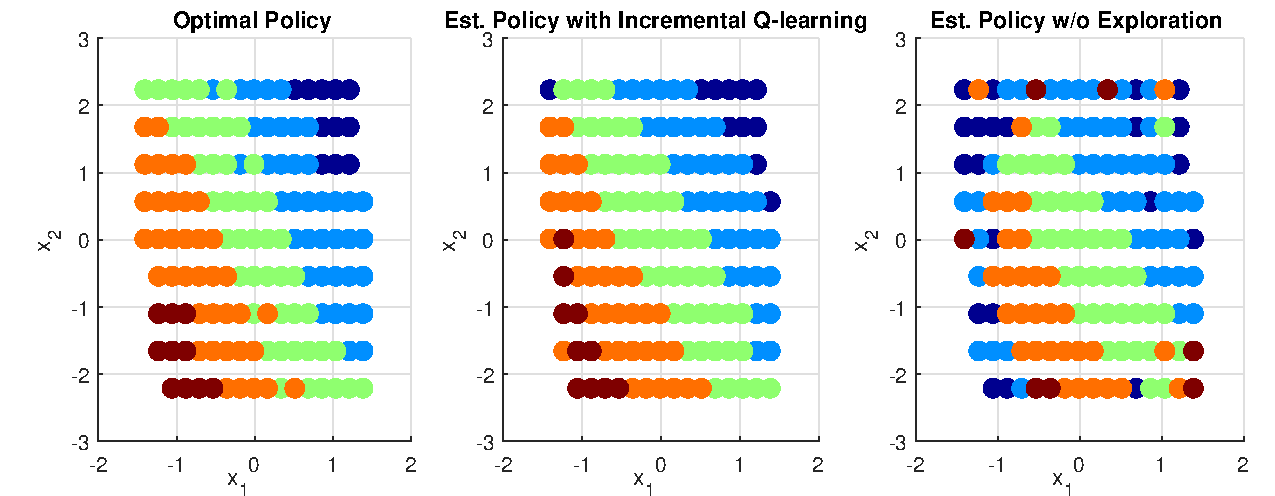
\includegraphics[width=0.8\paperwidth]{Policy}
\end{figure}
\end{frame}

\begin{frame}
\frametitle{Experimental Results}
\framesubtitle{Disturbance Estimation}
\begin{figure}
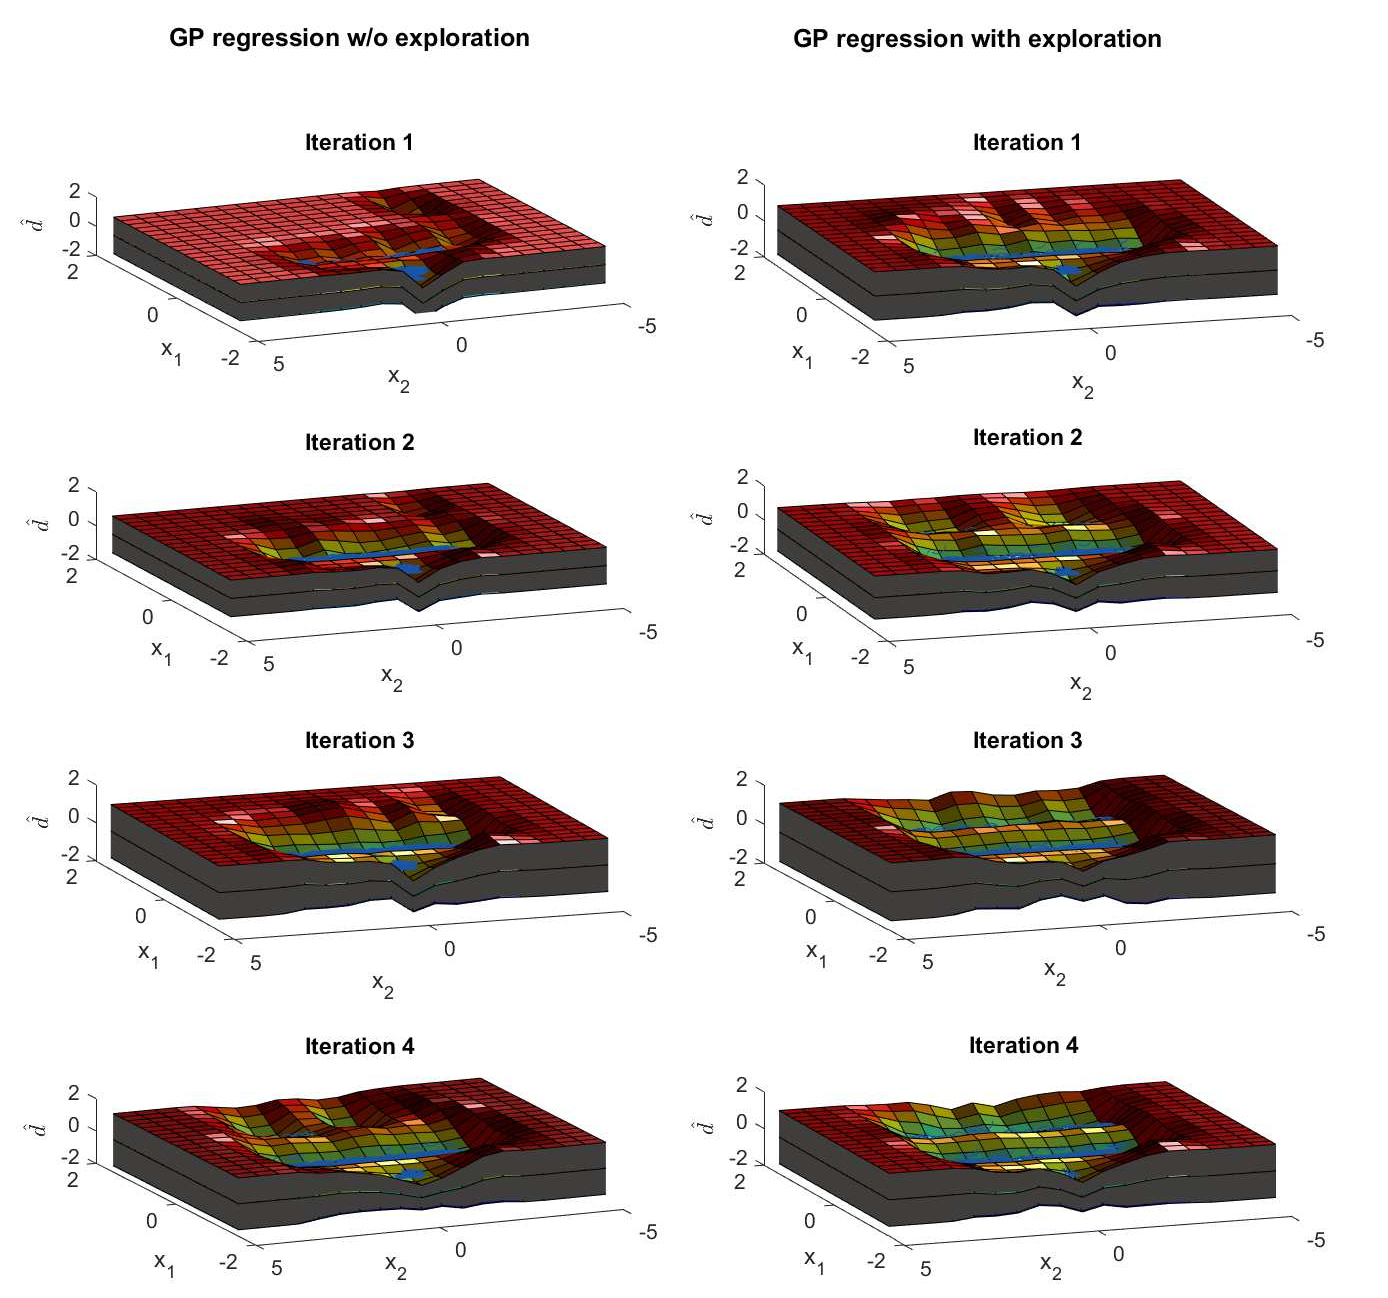
\includegraphics[width=0.8\paperwidth]{GP}
\end{figure}
\end{frame}

\begin{frame}
\frametitle{Experimental Results}
\framesubtitle{Simulation}
\begin{figure}
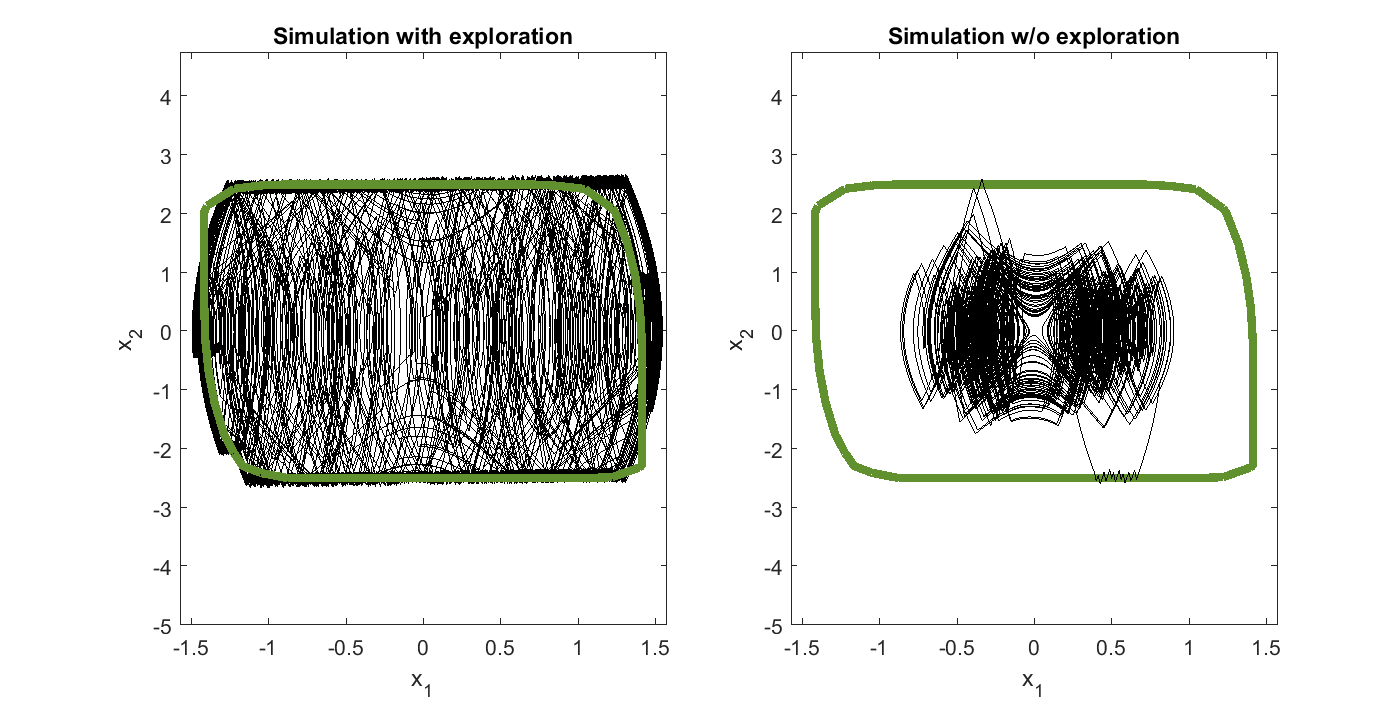
\includegraphics[width=0.8\paperwidth]{Simulation}
\end{figure}
\end{frame}

\begin{frame}
\frametitle{Conclusions and Future Work}
\begin{itemize}
\item Promising approach.
\item Better results by incorporating exploration.
\end{itemize}
\vspace{0.5cm}
Some work remains to be done:
\begin{itemize}
\item Joint design of safety and learning loop.
\item Recursive estimation of disturbance bounds.
\item Formal guarantees for the whole algorithm.
\makebox(1,1.2){\put(1,2\normalbaselineskip){%
               $\left.\rule{0pt}{1.2\normalbaselineskip}\right\}$ difficult}}
\end{itemize}
\end{frame}
\end{document}